% Compile with:
% latexmk -pvc -interaction=nonstopmode *Seminar.tex
\documentclass[aspectratio=169,10pt]{beamer}
%\documentclass[aspectratio=169,10pt,draft]{beamer}
\usetheme{UniBern}
\title{Tomographic imaging of fish}
\subtitle{Or how to image much, \emph{much} more teeth}
\author{David Haberthür}
\institute{Institute of Anatomy\\Universität Bern}
\date{January 18, 2024 | Seminar@Institute of Anatomy}

% Some often used abbreviations/commands
\newcommand{\everyframe}{333}% use only every nth frame for the animations
\newcommand{\imagewidth}{\columnwidth}% set global image width
\newcommand{\imageheight}{0.618\paperheight}% set global image heidht
\newlength\imagescale% needed for scalebars
\newcommand{\uct}{{\textmu}CT\xspace}% make our life easier
\newcommand{\eg}{e.\,g.\xspace}%
\newcommand{\ie}{i.\,e.\xspace}%

\usepackage[%
	backend=biber,
   	style=ieee,
	url=false,
	isbn=false,
    	citetracker=true,
    ]{biblatex}
\addbibresource{../../Documents/library.bib} % FastSSD, Windows or Mac works (on Linux/FastSSD we generated a 'Document' folder at the correct level and `ln -s ~/P/Documents/library.bib .` to it)
\usepackage{tikz}
	\usetikzlibrary{shadows,spy}
	\tikzset{shadowed/.style={preaction={transform canvas={shift={(1pt,-1pt)}},draw=ubRed}}}
\usepackage{shadowtext}
	\shadowoffset{1pt}
	\shadowcolor{ubRed}
\usepackage{pgfplots}
	\pgfplotsset{compat=newest}
\usepackage{microtype}
\usepackage[detect-all=true,
	range-phrase=--,
	range-units=single,
	per-mode=symbol,
	per-symbol=/]{siunitx}
\usepackage[absolute,overlay]{textpos}
\usepackage[showseconds=false,showzone=false]{datetime2}
\usepackage{gitinfo2}
\usepackage{xspace}
\usepackage{ccicons}
\usepackage{fontawesome5}
\usepackage[version=4]{mhchem}
\usepackage{animate}
\usepackage{listings}
	\lstset{basicstyle=\scriptsize\ttfamily}
	% highlight a line in listings: https://tex.stackexchange.com/a/58543/828
	% Including a crude workaround for recent versions of `listings`: https://tex.stackexchange.com/a/451538/828
	\makeatletter%
	\let\old@lstKV@SwitchCases\lstKV@SwitchCases%
	\def\lstKV@SwitchCases#1#2#3{}%
	\makeatother%
	\usepackage{lstlinebgrd}%
	\makeatletter%
	\let\lstKV@SwitchCases\old@lstKV@SwitchCases%
	\lst@Key{numbers}{none}{%
		\def\lst@PlaceNumber{\lst@linebgrd}%
		\lstKV@SwitchCases{#1}%
		{none:\\%
		left:\def\lst@PlaceNumber{\llap{\normalfont%
		\lst@numberstyle{\thelstnumber}\kern\lst@numbersep}\lst@linebgrd}\\%
		right:\def\lst@PlaceNumber{\rlap{\normalfont%
			\kern\linewidth{}\kern\lst@numbersep%
			\lst@numberstyle{\thelstnumber}}\lst@linebgrd}%
		}{\PackageError{Listings}{Numbers #1 unknown}\@ehc}}%
	\makeatother%
	% highlight a line in listings: https://tex.stackexchange.com/a/58543/828
\usepackage{pgfplotstable}
\usepackage{booktabs}
\usepackage{colortbl}
\usepackage{mathastext}
\usepackage{lipsum}

% change tikz font to slide font
% https://tex.stackexchange.com/a/33329/828
\usepackage[eulergreek]{sansmath}
\pgfplotsset{tick label style = {font=\sansmath\sffamily},
	every axis label = {font=\sansmath\sffamily},
	legend style = {font=\sansmath\sffamily},
	label style = {font=\sansmath\sffamily}
}

% Globally thicker lines in with tikz
% https://tex.stackexchange.com/a/206769/828
\tikzset{every picture/.style={thick}}

% Define a custom footer *with* progress bar, based on https://tex.stackexchange.com/a/59749/828
\makeatletter%
\def\progressbar@progressbar{}% the progress bar
\newcount\progressbar@tmpcounta% auxiliary counter
\newcount\progressbar@tmpcountb% auxiliary counter
\newdimen\progressbar@pbht%progressbar height
\newdimen\progressbar@pbwd%progressbar width
\newdimen\progressbar@rcircle% radius for the circle
\newdimen\progressbar@tmpdim% auxiliary dimension
\progressbar@pbwd=0.75\paperwidth%
\progressbar@rcircle=1.5pt%
\def\progressbar@progressbar{%
	\progressbar@tmpcounta=\insertframenumber%
	\progressbar@tmpcountb=\inserttotalframenumber%
	\progressbar@tmpdim=\progressbar@pbwd%
	\multiply\progressbar@tmpdim by \progressbar@tmpcounta%
	\divide\progressbar@tmpdim by \progressbar@tmpcountb%
		\hfill%
		\begin{tikzpicture}%
			\draw[ubGrey] (0,0) -- ++ (\progressbar@pbwd,0);%
			\draw[draw=ubRed,fill=ubGrey] (\the\dimexpr\progressbar@tmpdim-\progressbar@rcircle\relax,.5\progressbar@pbht) circle (\progressbar@rcircle);%
		\end{tikzpicture}%
		\hfill%
		bit.ly/ana-smnr-24\xspace|%
		\xspace v.~\href{https://github.com/habi/Talk.2024.AnatomyInternalSeminar/commit/\gitHash}{\gitAbbrevHash}\xspace|%
		\xspace p.~\insertframenumber/\inserttotalframenumber%
\vspace{0.5ex}%
}%
\addtobeamertemplate{footline}{}%
{%
	\begin{beamercolorbox}[wd=\paperwidth,center]{white}%
		\progressbar@progressbar%
	\end{beamercolorbox}%
}%
\makeatother%

% Acknowledge images just below them
% Based on https://tex.stackexchange.com/a/282637/828
\newcommand{\source}[2]{%
	% Print out (short) link under image, with small text
	\raisebox{-1.618ex}{%
		\makebox[0pt][r]{%
			\tiny\href{http://#1}{#1} #2%
			}%
		}%
	}%
\newcommand{\sourcecite}[2]{%
	% Cite (an image from) a reference
	\raisebox{-1.618ex}{%
		\makebox[0pt][r]{%
			\tiny From~\cite{#1}, #2%
			}%
		}%
	}%
\newcommand{\sourcelink}[3]{%
	% Make the source command an \href{link}{text}
	\raisebox{-1.618ex}{%
		\makebox[0pt][r]{%
			\tiny\href{#1}{#2}, #3%
			}%
		}%
	}%

% % References as footnotes at the bottom of the slides
% % https://tex.stackexchange.com/a/368760/828
% \makeatletter
% \renewcommand\@makefnmark{\xspace\hbox{\usebeamercolor[fg]{footnote mark}\usebeamerfont*{footnote mark}[\@thefnmark]}}
% \renewcommand\@makefntext[1]{\usebeamercolor[fg]{footnote mark}\usebeamerfont*{footnote mark}[\@thefnmark]\enspace\usebeamerfont*{footnote} #1}
% \makeatother

\makeatletter
\newbibmacro*{hypercite}{%
  \renewcommand{\@makefntext}[1]{\noindent\normalfont##1}%
  [\printfield{labelnumber}]\footnotetext{%
    \blxmkbibnote{foot}{%
    \printtext[labelnumberwidth]{%
      \printfield{prefixnumber}%
      \printfield{labelnumber}}%
    \addspace
    \fullcite{\thefield{entrykey}}}}}
\DeclareCiteCommand{\hypercite}%
  {\usebibmacro{cite:init}}
  {\usebibmacro{hypercite}}
  {}
  {\usebibmacro{cite:dump}}
\makeatother

% Reset footnote counter for every frame
\AtBeginEnvironment{frame}{\setcounter{footnote}{0}}
% Since we're using \footfullcite a lot, we remove most items to show from the citations, to keep the frames as clean as possible
\AtEveryCitekey{\clearfield{title}}
\AtEveryCitekey{\clearfield{journaltitle}}
% No "In:" http://tex.stackexchange.com/a/10686/828
\renewbibmacro{in:}{}
\AtEveryCitekey{\clearfield{volume}}
\AtEveryCitekey{\clearfield{number}}
\AtEveryCitekey{\clearfield{year}}
% No parentheses around the (now empty) year: https://tex.stackexchange.com/a/147537/828
\renewcommand{\bibopenparen}{\addcomma\addspace}
\renewcommand{\bibcloseparen}{\addcomma\addspace}
\AtEveryCitekey{\clearfield{pages}}
\AtEveryCitekey{\clearfield{issn}}

\begin{document}
% No footline on the title page
% http://tex.stackexchange.com/a/18829/828 helps us to achieve that
{%
	\setbeamertemplate{footline}{}%
	\begin{frame}[noframenumbering]
		\maketitle
	\end{frame}%
}

\begin{frame}
	\frametitle{Grüessech mitenang!}
	\begin{itemize}
		\item David Haberthür
		\begin{itemize}
			\item Physicist by trade
			\item \href{https://boris.unibe.ch/2619/}{PhD in high resolution imaging of the lung}, Institute of Anatomy, University of Bern, Switzerland
			\item Post-Doc I: \href{https://www.psi.ch/sls/tomcat/}{TOMCAT}, \href{https://www.psi.ch/sls/}{Swiss Light Source}, \href{https://www.psi.ch/}{Paul Scherrer Institute}, Switzerland
			\item Post-Doc II: \uct{} group, Institute of Anatomy, University of Bern, Switzerland.
		\end{itemize}
	\end{itemize}
\end{frame}

\section{Introduction}
\begin{frame}
	\frametitle{Grüessech from the \uct-group}
	\centering
	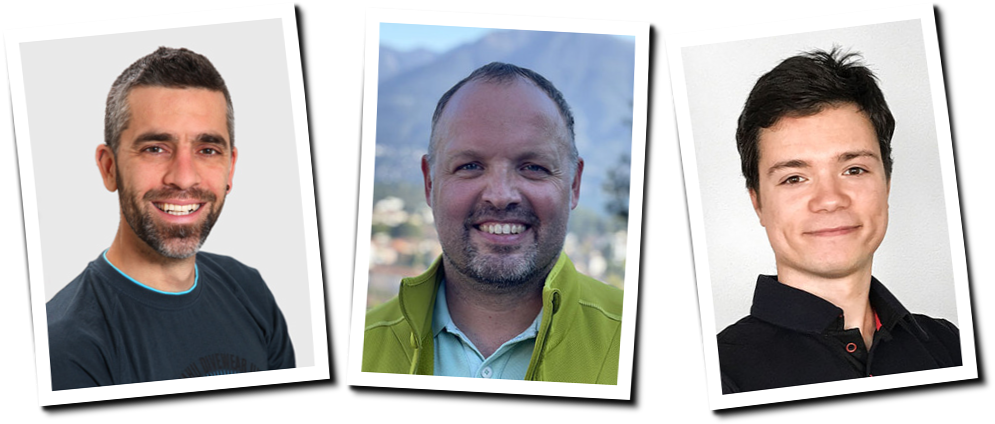
\includegraphics[height=\imageheight]{./media/team}
		\begin{columns}
		\hfill\begin{column}{0.33\textwidth}
			\centering%
			David{\color{ubRed!61.8}.}Haberthuer{\color{ubRed!61.8}@unibe.ch}%
		\end{column}
		\begin{column}{0.33\textwidth}
			\centering%
			Ruslan{\color{ubRed!61.8}.}Hlushchuk{\color{ubRed!61.8}@unibe.ch}%
		\end{column}
		\begin{column}{0.33\textwidth}
			\centering%
			Oleksiy{\color{ubRed!61.8}.}Khoma{\color{ubRed!61.8}@unibe.ch}%
		\end{column}\hfill%
	\end{columns}
\end{frame}

\renewcommand{\imagewidth}{\columnwidth}
\begin{frame}
	\frametitle{\uct-group}
	\begin{columns}
		\begin{column}{0.62\textwidth}
			\begin{itemize}
				\item microangioCT~\cite{Hlushchuk2019}
				\begin{itemize}
					\item Angiogenesis: heart, musculature~\cite{Nording2021} and bones
					\item Vasculature: (mouse) brain~\cite{Hlushchuk2020}, (human) nerve scaffolds~\cite{Wuthrich2020}, (human) skin flaps~\cite{Zubler2021} and tumors
				\end{itemize}
				\item Zebrafish musculature and gills~\cite{MesserliAaldijk2020}
				\item (Lung) tumor detection and metastasis classification~\cite{Trappetti2021}
				\item Collaborations with museums~\cite{Bochud2021} and scientist at UniBe~\cite{Halm2021,Kadlag2023} to scan a wide range of specimens, from human hearing bones to meteorites
				\item Automate \emph{all} the things!~\cite{Haberthuer2021,Haberthuer2023}
			\end{itemize}
		\end{column}%
		\begin{column}{0.38\textwidth}%
			\centering%
			\includegraphics<1>[width=\imagewidth]{./media/1172}%
			\only<1>{\source{brukersupport.com}{}}%
			\includegraphics<2>[width=\imagewidth]{./media/1272}%
			\only<2>{\source{bruker.com/skyscan1272}{}}%
			\includegraphics<3>[width=\imagewidth]{./media/2214}%
			\only<3>{\source{bruker.com/skyscan2214}{}}%
		\end{column}%
	\end{columns}%
\end{frame}


\section{Retrospection about teeth}
\begin{frame}
	\frametitle{Internal morphology of human teeth}
	\begin{columns}
		\begin{column}{0.5\textwidth}
			Collaboration with \href{https://www.zmk.unibe.ch/}{zmk bern – Zahnmedizinische Kliniken}~\hypercite{Haberthuer2021},~\hypercite{Wolf2021}
			\begin{itemize}
				\item 104 extracted human permanent mandibular canines
				\item Segmentation of teeth and root canal
				\item Numbers instead of just pretty images, unbiased characterization
				\item Reproducible and automated image analysis with \href{https://www.python.org/}{\faPython} in \href{https://jupyter.org/}{Jupyter}~\cite{Kluyver2016}
			\end{itemize}
		\end{column}%
		\begin{column}{0.5\textwidth}%
			\centering%
			\renewcommand{\imagewidth}{0.7\linewidth}
			\only<1>{%
			\pgfmathsetlength{\imagescale}{\imagewidth/2716}%
			\def\x{1678}% scalebar-x starting at golden ratio of image width of 2716px = 1678
			\def\y{2444}% scalebar-y at 90% of image height of 2716px = 2444
			\begin{tikzpicture}[x=\imagescale,y=-\imagescale]
				\node[anchor=north west, inner sep=0pt, outer sep=0pt] at (0,0) {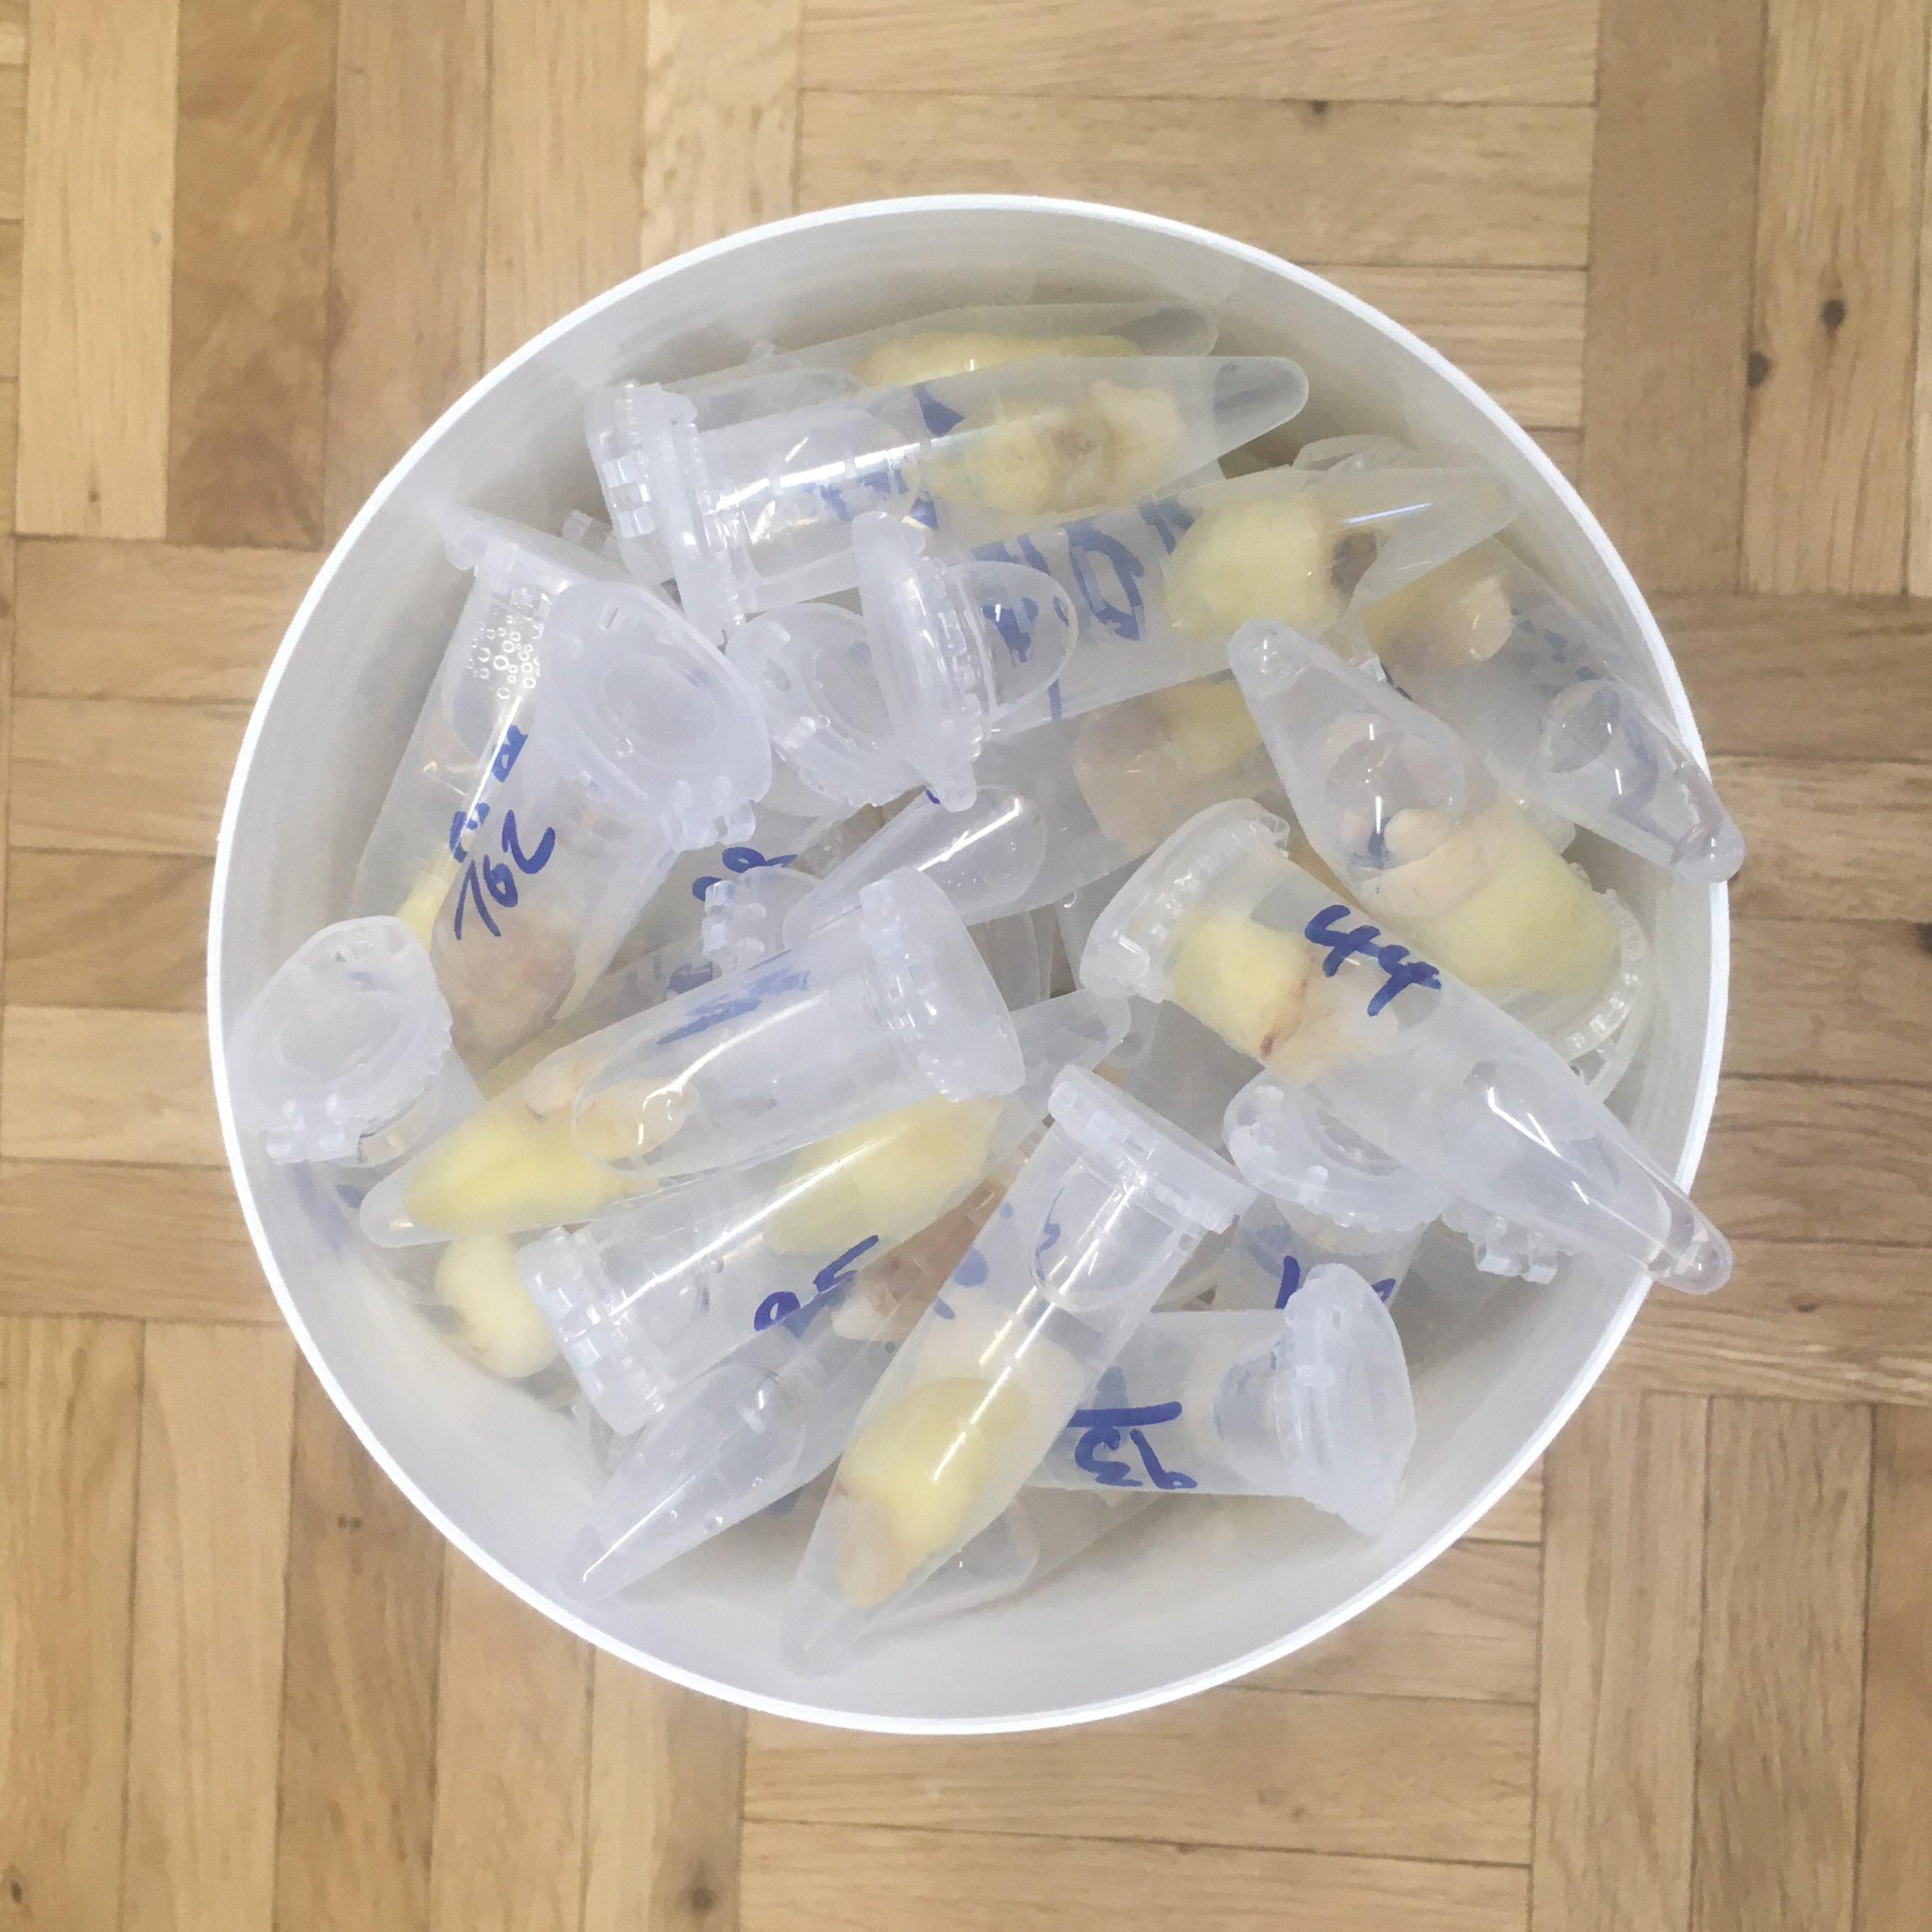
\includegraphics[width=\imagewidth]{./media/bucketofteeth}};
				% 2132.087px = 140.0mm -> 100px = 6566.337um -> 7.615px = 500um, 1.523px = 100um
				%\draw[|-|,blue,thick] (299,1340) -- (2430,1406) node [sloped,midway,above,fill=white,semitransparent,text opacity=1] {\SI{140.0}{\milli\meter} (2132px) TEMPORARY!};
				\draw[|-|,white,thick,shadowed] (\x,\y) -- (\x+761.5,\y) node [midway,above] {\shadowtext{\SI{5}{\centi\meter}}};
			\end{tikzpicture}%
			}%
			\renewcommand{\imagewidth}{\columnwidth}
		\end{column}%
	\end{columns}%
 \only<2>{
	 	\begin{tikzpicture}[remember picture,overlay]%
	 	\node at (current page.center) [shift={(0,-25pt)}]{%
		\animategraphics[autoplay,loop,width=\paperwidth,every=\everyframe]{24}{./media/ZMK/tooth045/transparent-slices-rcs/image0}{000}{457}%
	 		};%
	 \end{tikzpicture}%
	 }
\end{frame}

\section{Cichlids}
\begin{frame}
	\frametitle{Many more teeth, but from Cichlids}
			\begin{columns}
			\begin{column}{0.5\linewidth}
		 	Collaboration with team of \href{https://www.aqua.iee.unibe.ch/}{\emph{Aquatic Ecology \& Evolution}}, from the \href{https://www.iee.unibe.ch/}{Institute of Ecology and Evolution}
		\begin{itemize}
 		 		 	\item 133 Cichlids from Lake Victoria, East Africa
					\begin{itemize}
						\item Functional anatomy of the skulls and jaws
						\item<2-> \qtyrange{6}{18}{\centi\meter} in size
					\end{itemize}
					\item<7-> 375 scans in total
		 			\begin{itemize}
		 				\item<7-> 46 days of scanning time
		 				\item<7-> \qty{9.8}{\tera\byte} of raw data
		 				\item<7-> \qty{1.5}{\tera\byte} of reconstructions
		 				\item<7-> +\num{1000000} images
		 			\end{itemize}
		 		\end{itemize}
			\end{column}
			\begin{column}{0.5\linewidth}
				\centering
				\only<1>{%
					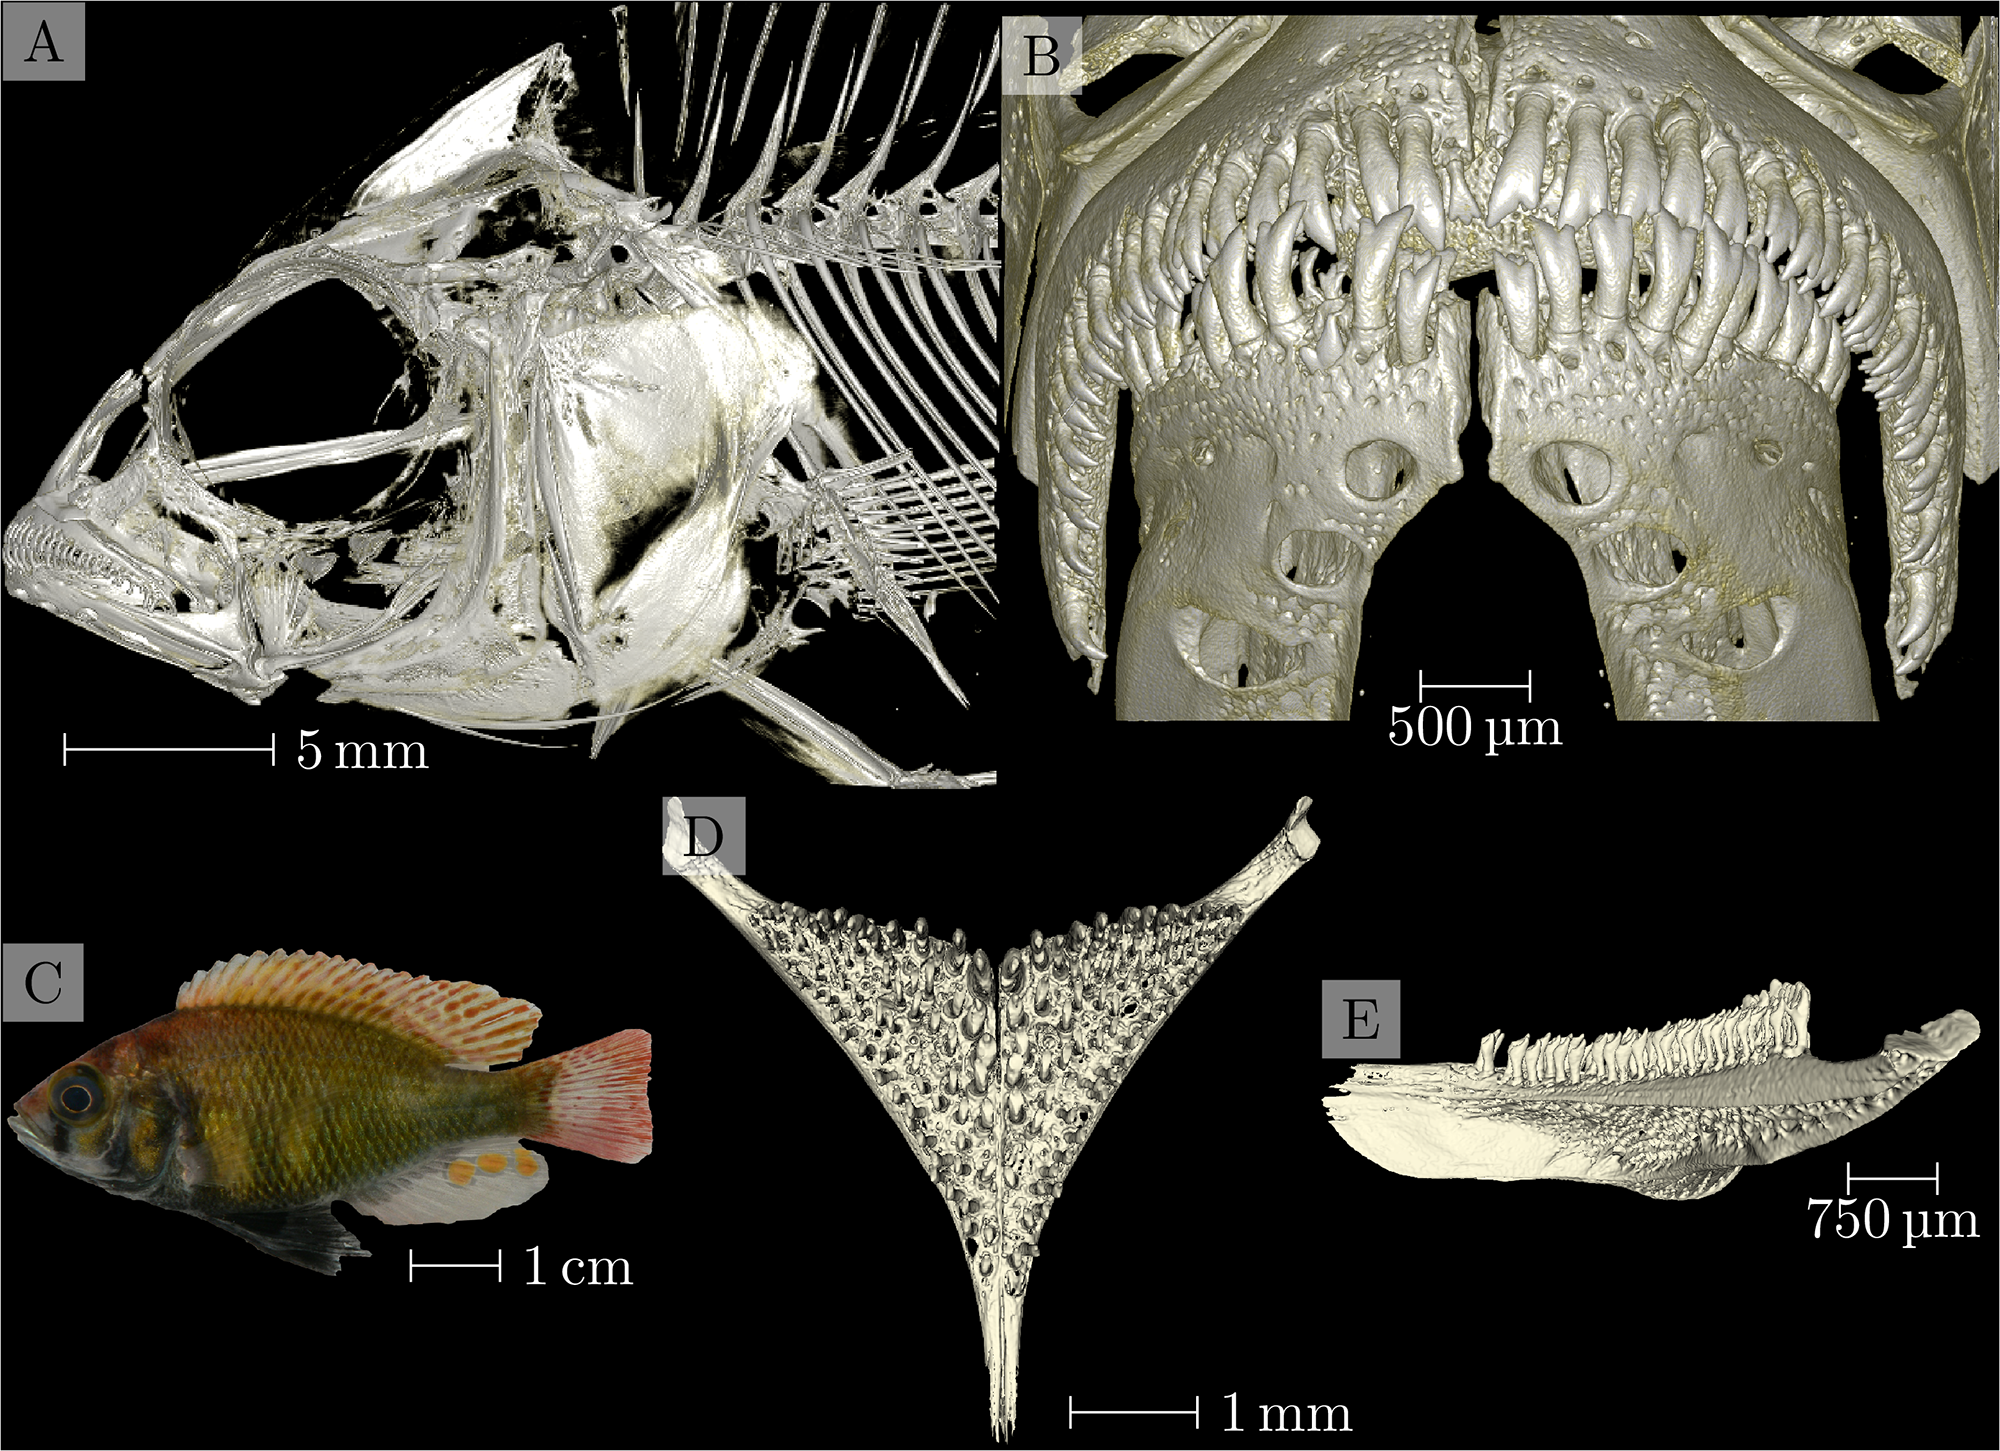
\includegraphics[width=\imagewidth]{./media/EAWAG/journal.pone.0291003.g001.png}%
					\sourcelink{https://journals.plos.org/plosone/article/figure?id=10.1371/journal.pone.0291003.g001}{doi:10.1371/journal.pone.0291003}{Fig.~1}%
					}%
				\includegraphics<2>[width=\imagewidth]{./media/EAWAG/lengths.plot.png}%
				\includegraphics<3>[width=\imagewidth]{./media/EAWAG/lengths.violinplot.png}%
				\includegraphics<4>[width=\imagewidth]{./media/EAWAG/lengths.boxplot.png}%
				\includegraphics<5>[width=\imagewidth]{./media/EAWAG/lengths.boxenplot.png}%
				\includegraphics<6>[width=\imagewidth]{./media/EAWAG/lengths.boxenplot.only.png}%
				\includegraphics<7>[width=\imagewidth]{./media/EAWAG/voxelsizes.png}%
			\end{column}
		\end{columns}
\end{frame}

 \begin{frame}
	\frametitle{Results}
	\centering
		\animategraphics[autoplay,loop,height=\imageheight,every=\everyframe]{24}{./media/EAWAG/animation.intro/104016}{0040}{0050}%
 \end{frame}

 \begin{frame}
	 \frametitle{Results}
 \centering
		 \animategraphics[autoplay,loop,height=\imageheight,every=\everyframe]{24}{./media/EAWAG/movie.104016_PJ/104016_PJ_00}{000}{236}%
 \end{frame}

 \begin{frame}
 	\frametitle{Data wrangling by example: Cichlids}
 	\centering
 	\includegraphics<1>[height=\imageheight]{./media/EAWAG/Otolither_104016_head_01_Overview}%
 	\includegraphics<2>[height=\imageheight]{./media/EAWAG/Otolither_104016_head_02_GrayValues}%
 	\includegraphics<3>[height=\imageheight]{./media/EAWAG/Otolither_104016_head_03_GrayValuesRegion}%
 	\includegraphics<4>[height=\imageheight]{./media/EAWAG/Otolither_104016_head_04_GrayValuesSmoothed}%
 	\includegraphics<5>[height=\imageheight]{./media/EAWAG/Otolither_104016_head_05_Peaks}%
 	\includegraphics<6>[height=\imageheight]{./media/EAWAG/Otolither_104016_head_06_Peaks_All}%
 	\includegraphics<7>[height=\imageheight]{./media/EAWAG/Otolither_104016_head_07_ExtractedRegions}%
 	\includegraphics<8>[height=\imageheight]{./media/EAWAG/Otolither_104016_head_08_ExtractedRegionsMIPs}%
 	\includegraphics<9>[height=\imageheight]{./media/EAWAG/Otolither_104016_head_09_ExtractedOtolithMasked}%
 	\only<10>{\href{https://htmlpreview.github.io/?https://github.com/habi/EAWAG-manuscript/blob/main/content/data/104016_Enterochromis_I_cinctus_St_E.head.rec.Otolith.Region.3D.html}{Exported 3D view}}%
 \end{frame}

 \subsection{Fish II}
 \renewcommand{\imageheight}{0.618\paperheight}% set global image height
 \begin{frame}
 	\frametitle{Data wrangling by example: Zebrafish}
 	\begin{columns}
 		\begin{column}{0.618\linewidth}
 			\begin{itemize}
 				\item Collaboration, part of a \emph{much} bigger story\footcite{Mercader2023}
 				\item Confirmation of results by \uct
 			\end{itemize}
 		\end{column}
 		\begin{column}{0.382\linewidth}
 			\centering
 			\includegraphics<1|handout:1>[height=\imageheight]{./media/cox7a/Cell_Fig3}%
 			\only<2|handout:2>{%
 				\lstinputlisting[linerange={2-4,15-15,17-19,28-30,36-37,40-40,44-44,53-54}]{./logfiles/ko02.log}%
 				}%
 		\end{column}
 	\end{columns}
 \note{The oxidative phosphorylation (OXPHOS) system is dynamic and the respiratory complexes (RCs) coexist with super-assembled quaternary structures called supercomplexes (SCs). How assembly occurs and the physiological role of supercomplex assembly is still under intensive investigation. The Cox7a family member Cox7a2l, also known as Scaf1, promotes CIII-CIV super assembly and energetic efficiency in zebrafish, mice, and humans. Here we studied the role of a second member of the Cox7a family, Cox7a1 in SC assembly and striated muscle physiology. We found that this protein drives CIV homodimer formation, which increases CIV activity. The substantial reduction in CIV2 formation led to a profound metabolic rearrangement with a consequent non-pathological loss of skeletal muscle performance and muscle mass not observed in cox7a2l. Ablation of Cox7a1 also rewired heart metabolism. While overall cardiac function was not affected, the absence of Cox7a1, but not Cox7a2l increased cardiac regenerative capacity. In sum, we describe a high specificity of Cox7a isoform in controlling OXPHOS assembly and muscle metabolism. While overall OXPHOS activity is modified, the loss of CIII-CIV heterodimer formation or CIV homodimer formation have very distinct metabolic and physiological consequences, highlighting the complexity of OXPHOS function and the importance of cox7a1 in striated muscle maturation.}
 \end{frame}

 \begin{frame}
 	\frametitle{Image analysis}
 	\centering
 	\includegraphics<1|handout:1>[height=\imageheight]{./media/cox7a/Overview}%
 	\includegraphics<2|handout:2>[height=\imageheight]{./media/cox7a/ko02_Cut}%
 	\includegraphics<3|handout:3>[height=\imageheight]{./media/cox7a/Histograms_Experiment}%
 	\includegraphics<4|handout:4>[height=\imageheight]{./media/cox7a/Volume_Boxplot}%
 \end{frame}


















\section{cox7a}
\begin{frame}
	\frametitle{More fish, but muscles}
			\begin{columns}
			\begin{column}{0.5\linewidth}
		 	Collaboration with \emph{Developmental Biology and Regeneration} group of Nadia Mercader Huber
		\begin{itemize}
 		 		 	\item 20 Zebrafish
					\begin{itemize}
						\item Influence of \emph{cox7a} on muscle volume
					\end{itemize}
		 		\end{itemize}
			\end{column}
			\begin{column}{0.5\linewidth}
				\centering
				Volume plot
			\end{column}
		\end{columns}
\end{frame}


\begin{frame}[allowframebreaks]
	\frametitle{References}
	\renewcommand*{\bibfont}{\scriptsize}
	\setbeamertemplate{bibliography item}{\insertbiblabel}
	\printbibliography{}
\end{frame}

\end{document}
